\subsection{VQA and QNN}

Hybrid techniques involving Quantum circuits and Classical optimisers have been proposed to overcome the restrictions of Noisy Intermediate-Scale Quantum (NISQ) \cite{brooksQuantumSupremacyHunt2019} devices. 
Those constraints are the absence of fault-tolerant design, restricted number of qubits per processor, and limited depth of executable quantum circuit. 
Moreover, quantum gates are static by design, which means every new data input into a quantum algorithm will produce a different quantum circuit.

Quantum circuits with trainable parameters can be utilised as reusable templates by Variational Quantum Algorithms (VQAs) \cite{cerezo2021variational}, which instantiate and refine their parameters for efficient execution on quantum computers.
It is also possible to rely on classical optimisers, which treat variational circuits as black boxes capable of yielding outputs from inputs and the circuit trainable parameters.

Consider a simple problem that we want to solve using VQA, given access to the training data.
The first step is to construct a \textit{cost function} $C$ used to search for an optimal set of circuit parameters, which is achieved by minimising the cost function during the training process.
Development of variational circuits can be simplified by composing the circuit templates called \textit{ansatze}. 
\textit{Ansatz} is the parameterized circuit that depends on a set of parameters $\theta$. We aim to train the ansatze by optimising the parameters $\theta$s so that the cost function $C$ reaches its minimum, thus satisfying:
\begin{equation}
    \theta^* = \underset{\theta}{\arg \min} \;C(\theta)
    \label{optimize theta with ansatz}
\end{equation}

In short, the cost function $C(\theta)$ is calculated using the Quantum computer, while the classical optimiser trains the parameters $\theta$. The Figure \ref{VQA diagram} elaborates on the VQA architecture and process in more detail.

\begin{figure}
    \centering
    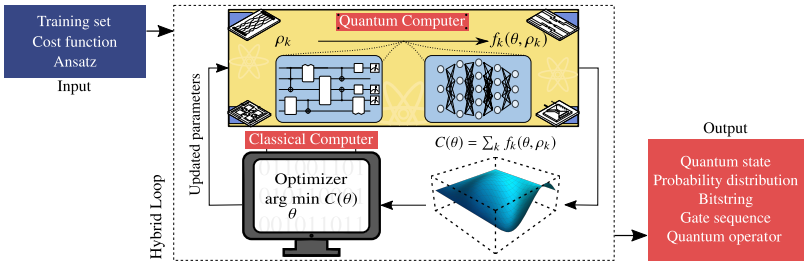
\includegraphics[width=\textwidth]{LiteratureReview/Appendices/vqadiagram.png}
    \caption{
    An illustrative diagram of VQA. 
    The algorithm is a hybrid loop that receives: 
    A cost function $C(\theta)$ for $\theta$ is a set of parameters that encodes the solution; 
    An ansatz that receives trainable parameter $\theta$ to solve the task;
    A set of training data $\{\rho_k\}$.
    We use the quantum computer to calculate the cost for each iteration, then use an optimization algorithm in a classical computer to find the global minima in the cost landscape $C(\theta)$ and thus satisfy the problem in Eq. (\ref{optimize theta with ansatz}).
    VQA's result is an approximation of the problem's solution, which can take forms as in the red box.
    Figure from Cerezo et al. \cite{cerezo2021variational}.
    }
    \label{VQA diagram}
\end{figure}

\subsubsection{The Cost Function}
Encoding the problem into a cost function is the first step to solving a problem using VQA \cite{cerezo2021variational}.
The cost function is equivalent to that used in classical machine learning. 
It maps the values of the trainable parameters $\theta$ into real values, which represent the measure of distance from an optimum solution.
For a function $f$ that receives input states $\{\rho_k\}$, observables $\{O_k\}$, and a parameterized circuit $U(\theta)$, the cost is expressed as:
\begin{equation}
    C(\theta) = f(\{\rho_k\}, \{O_k\}, U(\theta)) \;,
\end{equation}
or this form with a set of functions $\{ f_k \}$ and the square of a distance matrix given as its trace $Tr$:
\begin{equation}
    C(\theta) = \sum_k f_k \left(\Tr[ O_k U(\theta) \rho_k U^\dagger(\theta) ]\right) \;,
    \label{Cost function}
\end{equation}

There are some criteria in the construction of a cost function: 
(1) The cost function must be 'faithful' and 'operational meaningful', such that the minimum of $C(\theta)$ should correspond to the solution of the problem, and the lower cost function indicate a better solution in general;
(2) Cost function must be 'efficiently estimated' by measurement on a quantum computer and classical post-processing;
(3) The cost must be 'trainable', such that the parameters $\theta$ should be efficiently optimised.

\subsubsection{The Ansatzes}
\begin{figure} 
    \centerline{
        \Qcircuit @C=1em @R=0em {
        & \multigate{2}{U_1(\theta_1)}    & \multigate{2}{U_2(\theta_2)}    & \qw &        & & \multigate{2}{U_L(\theta_L)}   & \qw\\
        & \ghost{U_1(\theta_1)}           & \ghost{U_2(\theta_2)}           & \qw & \cdots & & \ghost{U_L(\theta_L)}          & \qw\\
        & \ghost{U_1(\theta_1)}           & \ghost{U_2(\theta_2)}           & \qw &        & & \ghost{U_L(\theta_L)}          & \qw
        \gategroup{1}{2}{3}{7}{.6em}{--}
        }
    }
    \centerline{$U(\theta)$}
    \centerline{}
    \centerline{}
    \centerline{
        \Qcircuit @C=1em @R=0em{
        & \multigate{1}{}   & \ctrl{2}  & \gate{}           & \qw \\
        & \ghost{}          & \qw       & \multigate{1}{}   & \qw \\
        & \gate{}           & \targ     & \ghost{}          & \qw
        \gategroup{1}{2}{3}{4}{.6em}{--}
        }
    }
    \centerline{$U_l(\theta_l)$}
    \caption{
        A diagram of a sample ansatz (above), the ansatz is a sequence of unitaries $U_l(\theta_l)$ (below).
        The unitary $U(\theta)$ receives parameters $\theta$ is expressed by $L$ layers of unitaries $U_l(\theta_l)$ for $l$ is the layer indices.
        Each $U_l(\theta_l)$ is a circuit composed of a mix of parameterized and unpasteurised gates.
    }\label{Ansatz diagram}
\end{figure}

The 'ansatze' is the parameterised circuit, parameterised unitary, or the "atomic" variational circuit.
In general, the location of parameters $\theta$ is determined by the ansatz form and can be trained to minimise the cost.
The ansatz structure can be defined based on the problem (called 'problem-inspired ansatzes) or a generic structure (called 'problem agnostic') that can be used without any relevant information available \cite{cerezo2021variational}.
The cost function in Eq. (\ref{Cost function}) encodes the parameters $\theta$ in a unitary $U(\theta)$ and applies to the input states of the circuit. 
The figure \ref{Ansatz diagram} shows that $U(\theta)$ can be expressed as a product of $L$ consecutive unitaries:
\begin{equation}
    U(\theta) = U_L(\theta_L) \cdots U_2(\theta_2) U_1(\theta_1)\;,
\end{equation}
with each layer:
\begin{equation}
    U_l(\theta_l) = \prod_m e^{-i\theta_m H_m} W_m
\end{equation}
for unparamaterized unitary $W_m$, Hermitian Operator $H_m$, and $\theta_l$ is the $l$-th element of $\theta$.

\subsubsection{The Gradients}
After defining the cost function and a suitable ansatz, we train the parameter $\theta = \{\theta_{l}\}$ to solve the problem in Eq. (\ref{optimize theta with ansatz}) \cite{cerezo2021variational}.
The cost function gradient helps the optimiser to find the global minima. 
Consider the cost function in Eq. (\ref{Cost function}), for a unitary that parameterizes rotation $e^{i \theta_l \sigma_{l}}$, where $\theta_l$ be the $l$-th element of $\theta$, $\sigma_l$ is a Pauli rotation operator. 
We can evaluate the gradient with the Parameter-shift rule:
\begin{equation}
    \frac{\partial C}{\partial\theta_l}
    = \sum_k \frac{1}{2 \sin{\alpha}} 
    \left( 
        \Tr[O_k U^\dagger(\theta_+) \rho_k U(\theta_+)] 
        - \Tr[O_k U^\dagger(\theta_-) \rho_k U(\theta_-)]
    \right) \;,
    \label{Parameter-shift rules}
\end{equation}
with $\theta_{\pm} = \theta \pm \alpha e_l$, $\alpha \in \mathbb{R}$ and $e_l$ is a vector such that its $l$-th position have the value of 1, or else 0.

Essentially, we can shift the $l$-th parameter by some amount $\alpha$, and Eq. (\ref{Parameter-shift rules}) will evaluate the gradient. 


\subsubsection{The Optimisers}
The accuracy of VQA greatly depends on the optimisation method.
Typically, we can achieve the solution by making successive moves along the gradient's direction.
This optimisation approach is within the scope of Stochastic Gradient Descent (SGD).
One example of SGD is the ADAM optimiser \cite{kingmaAdamMethodStochastic2014}, which can vary the size of the steps taken during optimisation to produce more efficient and precise results compared to the basic SGD.


\subsubsection{About QNN}
VQA is also the most widely used method for developing Quantum Neural Network (QNN) circuits. 
As a result, QNN inevitably inherited some of VQA's features and their flaws.
Many Quantum Machine Learning models suffer from the unsolvability due to \textit{Barren Plateaus} \cite{zhaoReviewQuantumNeural2021} that prevent the growth of circuit depth and lead training of parameters to a dead end.
When training a QNN framework with a large number of qubits, this phenomenon is likely to occur; the objective function becomes flat, making it nearly impossible to estimate the gradient, \cite{mccleanBarrenPlateausQuantum2018, zhaoAnalyzingBarrenPlateau2021} causing inefficiency in circuit training. 
We will discuss this matter in later sections.

Some architectures of QNN have been proposed to counter this problems, for example: 
Quantum Tensor Neural Network (QTNN) \cite{hugginsQuantumMachineLearning2019} which achieved a balance of computational efficiency and expressive power. 
The tensor network can reduce the required number of qubits to process high-dimensional data with powerful optimisation algorithms.
An alternative solution is to rely on Quantum Recurrent Neural Network (QRNN) which is constructed as a parameterised circuit \cite{takakiLearningTemporalData2021}, with some qubits being initialised and measured at each step while others memorise the past data.
The NISQ processors are also capable of delivering some other QNN models such as: 
Quantum Boltzmann Machine \cite{shinguBoltzmannMachineLearning2021, zoufalVariationalQuantumBoltzmann2021}, 
Quantum Perceptron \cite{kristensenArtificialSpikingQuantum2021}, 
Quantum Generative Adversarial Network \cite{dallaire-demersQuantumGenerativeAdversarial2018, lloydQuantumGenerativeAdversarial2018}. 
Studies have shown that QNN performance and trainability can be significantly higher than today's hardware's classical counterpart \cite{abbasPowerQuantumNeural2021, colesSeekingQuantumAdvantage2021}, and consequently may find some promising applications, for example, in breast cancer prediction \cite{liModelAlgorithmQuantuminspired2014} or image processing \cite{matsuiQubitNeuralNetwork2009}.

It is worth noting that Quantum Convolutional Neural Network (QCNN) does not exhibit Barren Plateaus \cite{pesahAbsenceBarrenPlateaus2021}.
Thus, trainability is guaranteed for QCNN under random initialisation.